\documentclass{report}

% The ams packages are required to insert any mathematical symbols that you may require
\usepackage{amsfonts}
\usepackage{amssymb}
\usepackage{amsmath}
\usepackage{amsthm}
% This package is used for embedding things like PDFs and JPEGs into your document
\usepackage{graphicx}
% This package is used for drawing pictures (such as trees)
\usepackage{tikz}
\usetikzlibrary{arrows,automata}
% These packages are used for adding pseudo-code to your document
\usepackage{algorithm2e}
\usepackage{algorithmic}
% This package is for if you require an appendix
\usepackage{appendix}

\usepackage{datetime}
\usepackage{fancyhdr}
\usepackage{semantic}
\usepackage[noload]{qtree}
\usepackage{comment}
\usepackage{pdflscape}
\usepackage{graphicx}
\usepackage[margin=1in]{geometry}
\usepackage{moreverb}
\usepackage{caption}
\usepackage{url}
\usepackage{layout}
\usepackage{subfig}
\usepackage{lineno}
\usepackage{bm}

\usepackage[annatar]{tengwarscript}

\newcommand{\arr}{\mathbb{R}}
\newcommand{\st}{\;\; st \;\;}
\newcommand{\nat}{\mathbb{N}}
\newcommand{\pr}{\mathbb{P}}
\newcommand{\vol}{\mbox{vol}}
\newcommand{\tengm}{\mbox{\Tmalta}}
%\newcommand{\tengm}{m}


\newtheorem{proposition}{Proposition}

\begin{document}

%\begin{titlepage}

\centering{\textsc{\huge{On the Properties of Monte Carlo Estimation of the Volume of a Convex Polytope}}}\\[1.5cm]

\centering{\textsc{\large{A Summer Project Funded by the University of Bristol's Prize Studentship Scheme}}}\\[1.5cm]

\begin{minipage}{0.4\textwidth}
\begin{flushleft} \large
\emph{Author:}\\
Tim Jones
\end{flushleft}
\end{minipage}
\begin{minipage}{0.4\textwidth}
\begin{flushright} \large
\emph{Supervisor:} \\
Dr. Rapha\"{e}l Clifford
\end{flushright}
\end{minipage}\\[1.5cm]

\vfill

\begin{abstract}
We evaluate a practical implementation of an efficient convex volume estimation algorithm, and tune its parameters such that they produce accurate results. We find that $2^5$ steps of a hit and run random walk is sufficient to produce adequately random points for shapes up to 10 dimensions and $2^{13}$ random points is enough to provide reasonable quality estimates of volume ratios. We then conclude by showing that for a convex polytope in 10 or more dimensions with 25 or more vertices, it is more efficient to use a randomised algorithm than to compute the volume exactly.
\end{abstract}

\vfill

Rendered on \today

\end{titlepage}

\clearpage

\newpage

\tableofcontents

\chapter{Introduction}

\section{Motivation and Goals}

The estimation of the volume of a convex shape in $n$ dimensions, $K$ is a long standing problem. Exactly calculating the volume of an arbitrary convex polytope is known to be \#P-hard, %cite
 but it has been shown by many authors %cite
that arbitrarily good estimates can be acquired by testing whether a polynomially bounded number of points fall within the shape. The order of this polynomial has been chipped away incrementally over many years until the most recent papers %cite simulated annealing and random walks
have successfully bounded the number of oracle queries to be within $O^{*}(n^4)$ and $O^{*}(n^5)$ respectively, stating that this brings the methods within the realms of a parctical implementation. Exact methods of volume computation exist and have been tested, but their scaling is measured in terms of the number of vertices and facets of the shape, not on the number of dimensions in which the shape exists. 

Our problem will be as follows. We will be given an inclusion oracle for $K$ which, on input of some point $\bm{x}$, will return either $\top$ if $\bm{x} \in K$ or $\bot$ otherwise. We also have the guarantee that $K$ is contained within a ball of known radius $R$, and that $K$ contains the unit ball. These guarantees are necessary, else we find ourselves in a situation where we may never even find the shape. We wish to construct an algorithm which, given such an oracle and an error measure $\varepsilon$, will, with high probability, return a value $v$ satisfying

$$
(1-\varepsilon)vol(K) \leqslant v \leqslant (1+\varepsilon)vol(K)
$$

In this study, we will test the various features of the $O^{*}(n^5)$ volume algorithm by implementing a version of it in ANSI C, using various statistical methods to estimate good values for relevant parameters, and finally compare its overall execution time to various exact methods of volume computation over various simplices. We will find that the theoretical upper bounds on most parameters are very loose indeed, and that in practice far smaller values are sufficient, resulting in significant savings on real-world execution time, however the assumption of a unit-time oracle proves impractical, and when more detailed information about the shape is available, an exact method is still usually faster. The theoretical performance of these algorithms is given in terms of the number of oracle queries made, ignoring the practicalities of actually building such an oracle.

\section{Preliminaries}
\subsection{Notation}

The quality of a volume estimation algorithm is usually measured using $O^{*}$ notation, which differs from $O$ notation in that poly-logarithmic factors and factors in terms of an accuracy parameter are suppressed. This has both benefits and drawbacks. The scaling of a poly-logarithmic factor is so small that we can justifiably neglect it for most exponents, and usually we do not scale the error parameter with the number of dimensions, however hiding this sort of information makes the actual practicalities of the algorithm harder to discern. An $O^{*}(n^4)$ algorithm may seem better than an $O^{*}(n^5)$, but due to hidden scaling with error parameters and logarithmic factors, may be slower in practice. $O^{*}$ notation is a useful tool, but is not a panacea.

We will denote the volume of some $n$-dimensional shape, $K$, by $\vol_n(K)$. Where a shape may exist in any number of dimensions, we will use $\vol_n$ to denote the volume of the $n$-dimensional version of that shape. Where the number of dimensions does not vary throughout an equation, we will neglect the $n$.

\subsection{Shapes}

We will call any continuous subset of $\arr^{n}$ a shape. A convex shape, $K$, is one which satisfies

$$
\forall u, v \in K, \lambda \in [0,1] \quad (\lambda u + (1-\lambda) v) \in K
$$

Such a combination of points is known as a convex combination. More intuitively, we say that $K$ is convex if any straight line segment between any two points in $K$ lies entirely within $K$. $K$'s boundary does not ``bow inwards".

We will denote by $B$ the unit ball, that is $B = \{x \in \arr^n \st ||x|| \leqslant 1\}$, and abuse notation slightly by donoting the ball of radius $R$ by $RB$. The ball of radius $RB$ is trivially the largest convex shape that will fit within the ball of radius $RB$. Its volume is easily calculable:

$$
\vol_n(RB) = \frac{\pi^{\frac{n}{2}}}{\Gamma(\frac{n}{2}+1)}R^n
$$

Where $\pi \approxeq 3.14$ denotes the circle constant, and $\Gamma = \int^\infty_0 t^{z-1}e^{-t} dt$ is Euler's gamma function, computable in closed form for integers and half-integers.

The convex hull of a set of points, denoted $h(P)$, is the set of points defined thus

$$
x \in h(P) \iff \exists u_1, u_2,...,u_k \in P, \lambda_1, \lambda_2, ..., \lambda_k  \in [0,1] \st x = \sum^{k}_{i=1} \lambda_i u_i \wedge \sum^{k}_{i=1} \lambda_i = 1
$$

Less formally, the convex hull of a set of points is the result of wrapping an elastic band around them and letting it snap tightly around them. All convex hulls are convex.

We will define the n-dimensional ice cream of radius $R$, $RI$ as the convex hull of $B$ and the point $(R,0,0,...0)$. Figure \ref{fig_ice_cream} should make the logic behind this name reasonably clear. The n-dimensional ice cream is important for this study because it is the smallest possible convex shape which contains $B$ and is tightly contained within $RB$. It will represent a pathological case for our estimation algorithms, however as the disjoint union of a capless ball and an n-dimensional cone, its volume, whilst non-trivial, is calculable in terms of the volume of an n-ball. The details can be found in Appendix \ref{app_ice_cream}.

$$
\vol_n(RI) = \frac{1-h}{n} \vol_{n-1}(rB) + \vol_n(B) - \left(\frac{1}{2}\vol_n(rB) I_{\frac{2rh-h^2}{r^2}}\left(\frac{n+1}{2}, \frac{1}{2}\right)\right) %Cite http://docsdrive.com/pdfs/ansinet/ajms/2011/66-70.pdf
$$
Where $h = \frac{1}{R}$, $r = \sqrt{1-\frac{1}{R^2}}$ and $I_x(a,b)$ is the incomplete beta function, defined thus:

$$
I_x(a,b) = \frac{\int^x_0 t^{a-1}(1-t)^{b-1}dt}{\int^1_0 t^{a-1}(1-t)^{b-1} dt}
$$

This function is the CDF of the beta distribution, and is available in various statistical packages.

\subsection{Markov Chains and Random Walks}

A Markov Chain is a triple, $(S,P,\bm{\delta})$, where $S$ is referred to as the state space, $P = (p_{st})_{s,t \in S}$ is the transition matrix and $\bm{\delta} = (\delta_s)_{s \in S}$ is the initial probability vector. A realisation of a Markov Chain is a sequence of states, $(x_i)_{i \in \nat}$ such that $\pr (x_0 = s)=\delta_s$, and $\pr(x_i = s_i | x_0 = s_0, ..., x_{i-1} = s_{i-1}) = \pr (x_i = s_i | x_{i-1} = s_{i-1})= p_{s_{i-1}s_{i}}$. We say that $\bm{\pi}$ is a stationary distribution of the Markov Chain if, given that $\bm{\delta} = \bm{\pi}$, the marginal probabilities $\pr(x_i = t) = \pi_t$ for all $i$ and $t$.  It is a standard result from probability theory that, if one can find a probability distribution $\bm{\pi}$ such that

$$
\forall s,t \in S, \quad \pi_s p_{st} = \pi_t p_{ts}
$$

Then $\bm{\pi}$ is the stationary distribution for the chain. It should be reasonably obvious that, if $p_{ij} = p_{ji}$ for all pairs of states, then $\bm{\pi}$ is a constant. If a stationary distribution exists for a chain, then, regardless of $\bm{\delta}$, $lim_{i-> \infty} \pr {x_i = s} = \pi_s$.

A random walk through a shape is a markov chain whose state space approximates the interior of a shape. We will use a random walk to sample uniformly at random from the inerior of a shape. By selecting a walk that satisfies $p_{ij} = p_{ji}$, we can can trace some number of steps from this walk, and return the state after some number of steps. The walk we use will be the Hit and Run Walk %cite Fast and Fun
which has been shown both theoretically and in practice to rapidly approach its stationary distribution, requiring a very small number of steps to produce good randomness. For a walk in the interior of $K$, starting at $\bm{x}_0$, the Hit and Run walk selects a line uniformly at random passing through $\bm{x}_0$ and contained entirely within $K$, then moves to a point uniformly distributed along this line. The number of times this needs to be repeated before a point becomes uniformly distributed in $K$ depends on $n$, and this will be discussed in section \ref{sec_mix}

Selecting the line through $\bm{x}_0$ can be accomplished by standard hyperspherical point picking %cite mathworld
followed by a binary search. We sample $n$ independent standard normal random variables to pick a random point on the surface of the $n$-dimensional unit hypersphere, $\bm{u}$, and define the line $\{\bm{x} | \bm{x} = \bm{x}_0 + \lambda \bm{u}, \lambda \in \arr \}$. Since we know that $K$ is contained within the ball of radius $R$, we know that $\bm{x}_0 + 2R\bm{u} \notin K$, and so can perform a bidirectional binary search to find $\overline{\lambda}$ and $\underline{\lambda}$ such that $\{\bm{x} | \bm{x} = \bm{x}_0 + \lambda \bm{u}, \lambda \in [\underline{\lambda}, \overline{\lambda}] \}$ is tightly contained within $K$. Selecting a $U(\underline{\lambda}, \overline{\lambda})$ random variable will then let us move to a uniformly random point on this line. Algorithm \ref{alg_samp} specifies this process.

\begin{algorithm}
\SetAlgoLined
\SetKwInOut{Input}{input}
\SetKwInOut{Output}{output}

\caption{An Algorithm for Generating a Uniformly Distributed Random Point in a Convex Shape}\label{alg_samp}
\Input{$\mathcal{O}_K$, an inclusion oracle for $K$, $n$, the number of dimensions in which $K$ exists, $R$, the radius of $K$, $n_s$, the number of steps to take before returning, and $\theta$, an accuracy parameter}
\Output{$\bm p$, a point in $K$ randomly distributed to be near uniform on $K$}

\Begin{
	${\bm p} <- 0$ \\
	\For{$i <- 1$ \KwTo $n_s$}{
		${\bm \delta} <-$ random\_direction \\
		$\overline{\lambda}' <- {\bm p} + 2R {\bm \delta}$ \\
		$\overline{\lambda}  <- 0$ \\
		$\underline{\lambda}' <- {\bm p} - 2R {\bm \delta}$ \\
		$\underline{\lambda}  <- 0$ \\
		\While{$\overline{\lambda}' - \overline{\lambda} > \theta$}{
			\uIf{${\bm p} + \frac{\overline{\lambda} + \overline{\lambda}'}{2}{\bm \delta} \in K$}{
				$\overline{\lambda}  <- \frac{\overline{\lambda} + \overline{\lambda}'}{2}$
			}\Else{
				$\overline{\lambda}' <- \frac{\overline{\lambda} + \overline{\lambda}'}{2}$
			}
		}
		\While{$\underline{\lambda}' - \underline{\lambda} > \theta$}{
			\uIf{${\bm p} + \frac{\underline{\lambda} + \underline{\lambda}'}{2}{\bm \delta} \in K$}{
				$\underline{\lambda}  <- \frac{\underline{\lambda} + \underline{\lambda}'}{2}$
			}\Else{
				$\underline{\lambda}' <- \frac{\underline{\lambda} + \underline{\lambda}'}{2}$
			}
		}
		$\lambda <-$uniform$(\underline{\lambda}, \overline{\lambda})$\\
		${\bm p} <- {\bm p} + \lambda {\bm \delta}$
	}
	\KwRet $\bm p$
}
\end{algorithm}

In the implementation, uniform random numbers are selected via the mersenne twister, and normally distributed random numbers are selected with the ziggurat algorithm. These two methods are known to generate high quality random numbers quickly.

\subsection{The Volume Estimation Algorithm}

The algorithm we will use follows %lovasz paper
with three differences. Rather than generating random points using the ball walk, we generate points with Hit and Run, which previous experimental results show mixes significantly faster than the ball walk. Rather than using $2$ as the base for our exponents, we use $e$.

To estimate the volume of some shape, $K$, we choose a sequence of shapes, $K_0 \subseteq K_1 \subseteq ... \subseteq K_p$, such that the volume of $K_0$ can be computed easily, $K_p = K$, and we can estimate the ratios $\frac{vol(K_{i+1})}{vol(K_i)}$ easily. For our algorithm, we will chose the shapes $K_i = (e^{i/n}B) \cap K$ for $i = 0, ..., n \log (R)$. Since $B \subseteq K \subseteq RB$, this satisfies our first two conditions. We can then estimate the ratios by sampling uniformly at random from $K_i$ and counting the number of points which fall into $K_{i-1}$. Modifying an oracle that samples from $K$ such that it samples from $K_i$ is fairly easy, and ratio of volumes can be estimated as the fraction of uniformly generated random points in $K_i$ that fall into $K_{i-1}$. Algorithm \ref{alg_vol} specifies this in pseudocode.

\begin{algorithm}
\SetAlgoLined
\SetKwInOut{Input}{input}
\SetKwInOut{Output}{output}

\caption{An Algorithm for Estimating the Volume of a Convex Shape}\label{alg_vol}
\Input{$\mathcal{O}_K$, an inclusion oracle for $K$, $n$, the number of dimensions in which $K$ exists, $R$, the radius of $K$, and $n_p$, a number of points to use per thread}
\Output{$v$, an estimate of $vol(K)$}

\Begin{
	$n_s <- n \lceil \ln (R) \rceil$ \\
	$v <-\vol_n(B)$ \\
	$K_0 <- B$
	\For{$i <- 1$ \KwTo $n_s$}{
		$K_i <- e^\frac{i}{n}B \cap K$ \\
		$n_{in} <- 0$
		\For{$j <- 1$ \KwTo $n_p$}{
			$p <-$ generate\_point$(K_i)$ \\
			\If{$p \in K_{i-1}$}{
				$n_{in} <- n_{in} + 1$
			}
		}
		$v <- \frac{n_s v}{n_{in}}$
	}
	\KwRet $v$
}
\end{algorithm}

\subsection{Neglected Details}

This field is very well researched, and not every part of this research can be accounted for in this study.

Firstly, when sampling a point, the sampling algorithm is actually capable of starting from any arbitrary location. The line ${\bm p} <- 0$ from algorithm \ref{alg_samp} can instead by a previously generated point, passed as a parameter, to be perturbed by the random walk. The algorithms in the literature tend to use the previously generated point as a starting point, thus providing a ``warm start" to the random walk. Preliminary experiments showed that this produced random numbers of lower quality than starting from $0$ every time.

The literature assumes that, if $K \subseteq RB$, then $R \in O^{*}(\sqrt{n})$. If this is not the case, then it is fairly easy to transform space such that it is, for some predetermined constant factors hidden by the $O$ notation. In this study, we will ignore this by simply generating shapes for which $R = \sqrt{n}$ in every case. This transformation also includes a translation such that te centre of $K$'s mass is at the origin. This provides a useful technical tool to make the analysis easier, but is not necessary for the algorithms to be correct. Similarly, we neglect the step of adjusting the size of the shape such that the covariance matrix of its uniform distribution is the identity, though we will revisit this later for some of the statistical tests.

\chapter{Experiments}

\section{Mixing time}\label{sec_mix}

Our first experiment will attempt to bound the mixing time of the Hit and Run random walk in a convex shape. The hit and run walk is known to mix rapidly %cite hit and run is fast and fun, as well as Vempala's proof of warm start-ness
in the sense that the number of steps needed for the walk to reach a uniform ditribution is $O^{*}(n^2)$, however this result actually shows that the walk can only be guaranteed to mix after over $10^{10} n^2$
steps. A hit and run step requires the generation of $n$ uniformly distributed random numbers, which is already a difficult task. Performing $10^{10} n^2$ steps, then, is very much infeasible on modern hardware.

We shall judge the walk to be well-mixed if 1,000 independent points generated by the walk with a fixed starting point at the origin pass a $\chi^2$ test at the 5\% level against the null hypothesis that the points are identically distributed to a set of 1,000 points sampled by a method guaranteed to generate uniform points, but which may be somewhat slower. It is not clear which shape is likely to constitute a pathological case for the hit and run walk; the ice cream has the smallest volume, and so in a sense fewer points need to be chosen from, but also has the tighest possible corner, in which the walk is most likely to get stuck. By contrast, the ball has the largest volume and no corners. We will test both shapes. Uniformly distributed random points can be generated from a ball fairly easily, and uniform random points can be generated from an ice cream by simple rejection sampling. To keep our search reasonably short,  we will restrict ourselves to only testing numbers of steps equal to natural powers of 2.

%Actual write up of results goes here as soon as I can de-dumb the chi squared tests. Kolmogorov-Smirnov tests may have to 

From this, we can see that the number of steps needed to generate a uniform random point is still reasonably large, but nowhere near the upper bound of $10^10$. This is relieving, and we will use these numbers of steps for each dimension in the sequel.


\section{Threads per stage}\label{sec_error}

We will now see how the number of threads per phase influences the accuracy of an estimate. In the paper describing our particular estimation method, it is stated that, for an n-dimensional shape, in order to achieve an error of $\varepsilon$, we should use $400\frac{n\log n}{\varepsilon^2}$ threads per stage. This, again, is an upper bound, and we would like to show that it is loose. We shall vary the number of threads used per stage, and see how the distribution of estimates varies with this value. As before, we will use both the ice cream and the ball to respectively maximise and minimise the ratios between successive shapes. Our analysis here will be largely visual, since any returned value from this algorithm might be considered valid for a sufficiently large value of epsilon.


\section{Computation Time for Convex Shapes}\label{sec_time}

It's now time to test the practicalities of this algorithm on a series of convex shape, against already established methods of exact volume computation. The code used for comparison is the same as that used in %cite exact methods
and was run over a series of randomly generated convex shapes. Each shape is the convex hull of the box $[-1,1]^n$, and some variable number of points on the ball of radius $\sqrt n$. We will randomly generate series of shapes in each dimension, increasing the number of points on the hull, and seeing how this affects the time for a volume estimation to complete to a precision of $\varepsilon = 0.1$.

All experiments were conducted on the same hardware and in the same operating system, using the same time metric. The processor is an Intel i5-2500k in a Gigabyte Z68AP-D3 motherboard, connected to 8 GiB of 1,600 MHz dual-challen DDR3 RAM. The programs were both compiled onto a 64-bit install of Ubuntu 12.04 virtualised by Oracle VM Virtualbox with access to 2GiB of RAM. Each time is measured in elapsed clock cycles divided by the number of clocks per second. Using this processor time removes the possibility of error due to other running processes. Neither program is designed to exploit any more than a single processor core.

The oracle is implemented with a linear programming solver, which tests whether a queried point can be written as a convex combination of the points on a hull. The LP solver used is Gurobi, which is the fastest LP solver currently available.


Unfortunately, despite the high-speed LP solver, the oracle queries are very much not free. The majority of our time in this case is spent answering oracle queries, not performing the auxillary operations. %Talk about scaling of answering oracle queries - if they scale as badly as solving LPs, we're basically wasting our time here. Otherwise, eventually this will be badass

\appendix
\chapter{The Ice Cream} \label{app_ice_cream}

The $n$-dimensional ice cream of radius $R>1$, denoted $RI$ is the convex hull of the unit ball and the point $(R,0,0...,0)$. In this section, we will simply prove that its volume is

$$
\vol_n(RI) = \frac{R-h}{n} \vol_{n-1}(rB) + \vol_n(B) - \left(\frac{1}{2}\vol_n(rB) I_{\frac{2rh-h^2}{r^2}}\left(\frac{n+1}{2}, \frac{1}{2}\right)\right)
$$

With $h = \frac{1}{R}$, $r = \sqrt{1-\frac{1}{R^2}}$ and $I_x(a,b)$ is the incomplete beta function, defined thus:

$$
I_x(a,b) = \frac{\int^x_0 t^{a-1}(1-t)^{b-1}dt}{\int^1_0 t^{a-1}(1-t)^{b-1} dt}
$$

We will show that the shape can be written as the union of two disjoint sets. Let

$$
S = B \cap \left\{{\bm x} | x_1 \leqslant \frac{1}{R}\right\}
$$

And

$$
W = \left\{{\bm x} + \left(\frac{1}{R}, 0, ..., 0\right) | x_1 > 0 \; \wedge \; \sum^{n}_{i=2} x_i^2 < \left(\frac{\sqrt{1-R^{-2}}}{R-R^{-1}} x_1\right)^2 \right\}
$$

We will call $S$ the scoop, and is the spherical part of the ice cream near the origin, and $W$ the wafer, the conical part nearer to the point $(R,...,0)$. These two shapes are clearly disjoint, so the volume of the ice cream is the sum of the volumes of the cone and the wafer. We will show that these shapes partition the ice cream by showing that any line tangent to the unit ball through $(R,0,...,0)$ touches the ball at a point whose first coordinate is $\frac{1}{R}$.  The set of points touching the surface of an $n$-ball whose first coordinate is $\frac{1}{R}$ is an $(n-1)$-ball of radius $\sqrt{1-R^{-2}}$, and the distance from this surface to $(R,0,...,0)$ is $1-\frac{1}{R}$. The convex hull of points on an $n-1$ dimensional surface with a point normal to the surface is an $n$-dimensional hypercone. This hypercone is the wafer, the remainder is the scoop. Most of this will manifest as simple but non-obvious geometry, so it is worth describing fully.

\begin{proposition}
A line tangent to the unit $n$-ball that passes through $(R,0,...,0)$ intersects the surface of the $n$-ball at a point whose first coordinate is $\frac{1}{R}$ at a distance $\sqrt{1-\frac{1}{R^2}}$ from the line from the origin to $(R,0,...,0)$
\end{proposition}

The situation is as depicted in figure \ref{fig_ice_cream_annotated}. $O$ is the origin, $B$ is the point $(R,0,...,0)$, and $A$ is any point on the surface of the unit $n$-ball such that $AB$ is tangent to the surface. $OAB$ is a right angle. $C$ is the point such that $O$, $C$ and $B$ are colinear, and $ACB$ is a right angle. Since $OAB$ is a right angled triangle, $|AB| = \sqrt{R^2-1}$. From the law of sines, $\sin(AOB) = \frac{\sqrt{R^2-1}}{R}$, so $\cos(AOB) = \frac{1}{R}$, so $|OC| = \frac{1}{R} = h$, and $|AC| = \sqrt{1-\frac{1}{R^2}} = r$, as required.

We also have that $|CB| = R-h$, and that the points on the surface of the unit ball whose first coordinate is $h$ is an $(n-1)$-ball of radius $r$. This tells us that the wafer is an $n$-dimensional hypercone of height $R-h$ and whose base is the $(n-1)$-ball of radius $r$.

\begin{figure}
\centering
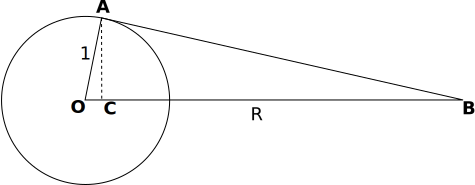
\includegraphics{./images/ice_cream_annotated.pdf}
\caption{Annotated components of an ice-cream, projected onto the 2-d plane. Points are in bold font, and variables in italic.}
\label{fig_ice_cream_annotated}
\end{figure}

\begin{proposition} \label{prop_vol_wafer}
The volume of the wafer is $\frac{R-h}{n} \vol_{n-1}(rB)$
\end{proposition}

The set of points in the wafer at a distance of $t$ from point $B$ is exactly the set of points in the $(n-1)$-ball of radius $\frac{rt}{R-h}$, so

\begin{align*}
\vol(W)
&= \int^{R-h}_{0} \vol_{n-1}\left(\frac{t}{R-h}rB\right) dt \\
&= \frac{1}{R-h}^{n-1} \vol_{n-1}(rB) \int^{R-h}_0 t^{n-1}dt \\
&= \frac{R-h}{n} \vol_{n-1}(rB)
\end{align*}
As required.

\begin{proposition} \label{prop_vol_scoop}
The volume of the scoop is $\vol_n(B) - \left(\frac{1}{2}\vol_n(rB) I_{\frac{2rh-h^2}{r^2}}\left(\frac{n+1}{2}, \frac{1}{2}\right)\right)$
\end{proposition}

The scoop is exactly a unit hypersphere without a hyperspherical dome. The volume of an $n$-spherical dome of height $h$, radius $r$ is $\frac{1}{2}\vol_n(rB) I_{\frac{2rh-h^2}{r^2}}\left(\frac{n+1}{2}, \frac{1}{2}\right)$, as proven in \cite{Li11}, so the volume of the scoop is $\vol_n(B) - \left(\frac{1}{2}\vol_n(rB) I_{\frac{2rh-h^2}{r^2}}\left(\frac{n+1}{2}, \frac{1}{2}\right)\right)$

Combining propositions \ref{prop_vol_wafer} and \ref{prop_vol_scoop}, we have the volume of the entire ice cream.


\end{document}